%!TEX root = main.tex
%=================TD functions==================
\def\boldcommandlist{\@elt OP,\@elt OPs,}
\def\@elt#1,{%
 \expandafter\def\csname#1\endcsname{\textbf{#1}\xspace}
}
\boldcommandlist

\def\topColorList{\@elt TOP,\@elt TOPs,}
\def\@elt#1,{%
 \expandafter\def\csname#1\endcsname{\textcolor{TOP}{\textbf{#1}}\xspace}
}
\topColorList

\def\chopColorList{\@elt CHOP,\@elt CHOPs,}
\def\@elt#1,{%
 \expandafter\def\csname#1\endcsname{\textcolor{CHOP}{\textbf{#1}}\xspace}
}
\chopColorList

\def\sopColorList{\@elt SOP,\@elt SOPs,}
\def\@elt#1,{%
 \expandafter\def\csname#1\endcsname{\textcolor{SOP}{\textbf{#1}}\xspace}
}
\sopColorList

\def\datColorList{\@elt DAT,\@elt DATs,}
\def\@elt#1,{%
 \expandafter\def\csname#1\endcsname{\textcolor{DAT}{\textbf{#1}}\xspace}
}
\datColorList

\def\matColorList{\@elt MAT,\@elt MATs,}
\def\@elt#1,{%
 \expandafter\def\csname#1\endcsname{\textcolor{MAT}{\textbf{#1}}\xspace}
}
\matColorList


\def\compColorList{\@elt COMP,\@elt COMPs,}
\def\@elt#1,{%
 \expandafter\def\csname#1\endcsname{\textcolor{COMP}{\textbf{#1}}\xspace}
}
\compColorList

\def\redcommandlist{\@elt missingImage,}
\def\@elt#1,{%
 \expandafter\def\csname#1\endcsname{\textcolor{red}{\textbf{#1}}\xspace}
}
\redcommandlist

%===============================================

\chapter{Lecture 3}

\section{Notes}

\begin{itemize}
	\item \SOPs explanations: Transform, Merge, Copy, Subdivide, Group
	\item Geometry Types, SOP to \DAT for inspection
	\item Panel Interaction + Generative Design Example
	\item Instancing, SOP to \CHOP
	\item Oscilloscope
	\item Trail \CHOP + instancing


\end{itemize}


\begin{figure}[H]
	\centering
	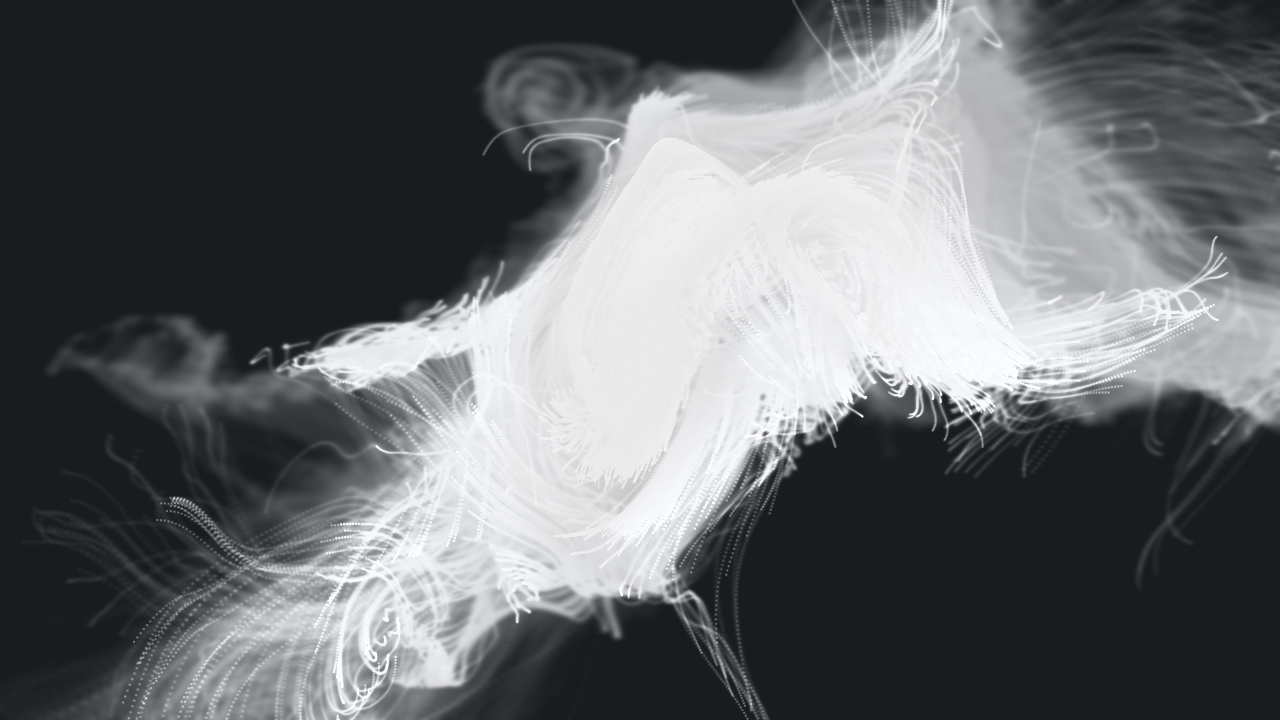
\includegraphics[width=\textwidth]{img/particle2.png}
	\caption[Particle system with feedback]
	{Particle system with feedback}
	\label{fig:label}
\end{figure}


\begin{figure}[H]
  \centering
  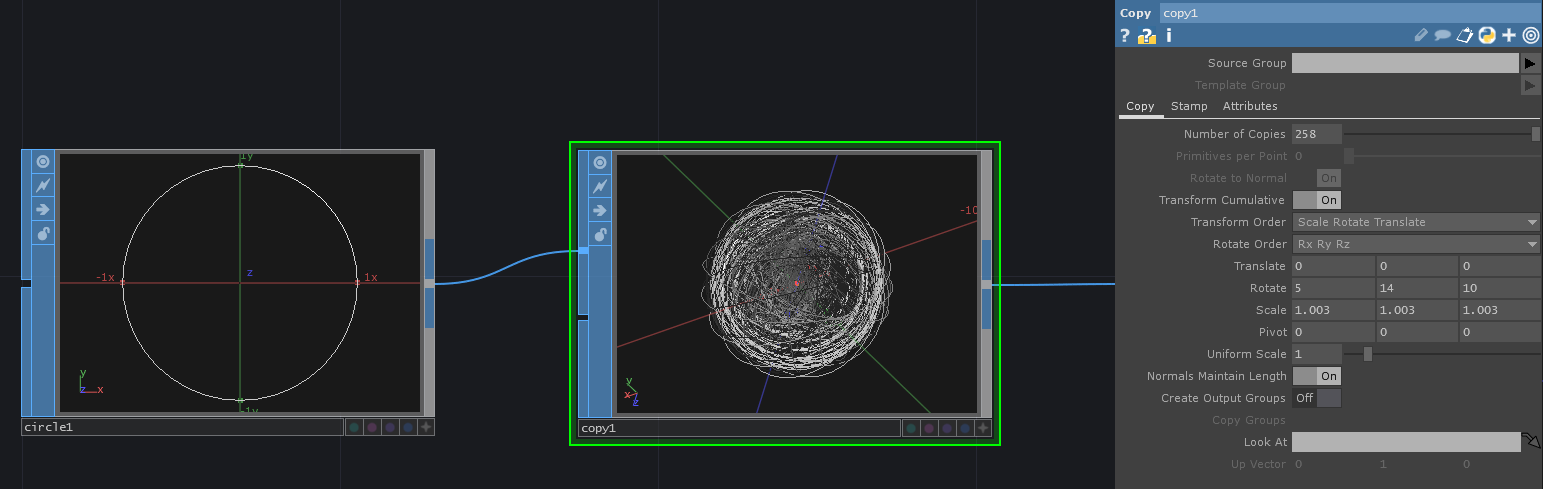
\includegraphics[width=\textwidth]{img/copySop.PNG}
  \caption[shortCaption]
  {CAPTION MISSING}
  \label{fig:label}
\end{figure}




\begin{figure}[H]
  \centering
  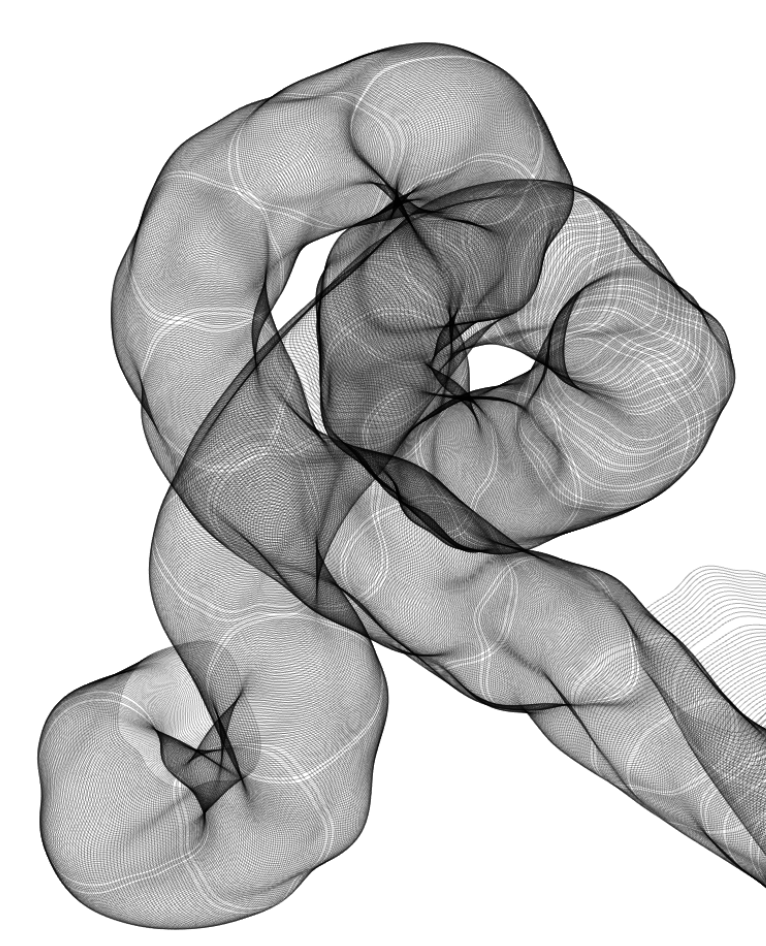
\includegraphics[width=10cm]{img/ggForms01.PNG}
  \caption[shortCaption]
  {CAPTION MISSING}
  \label{fig:label}
\end{figure}


\begin{figure}[H]
  \centering
  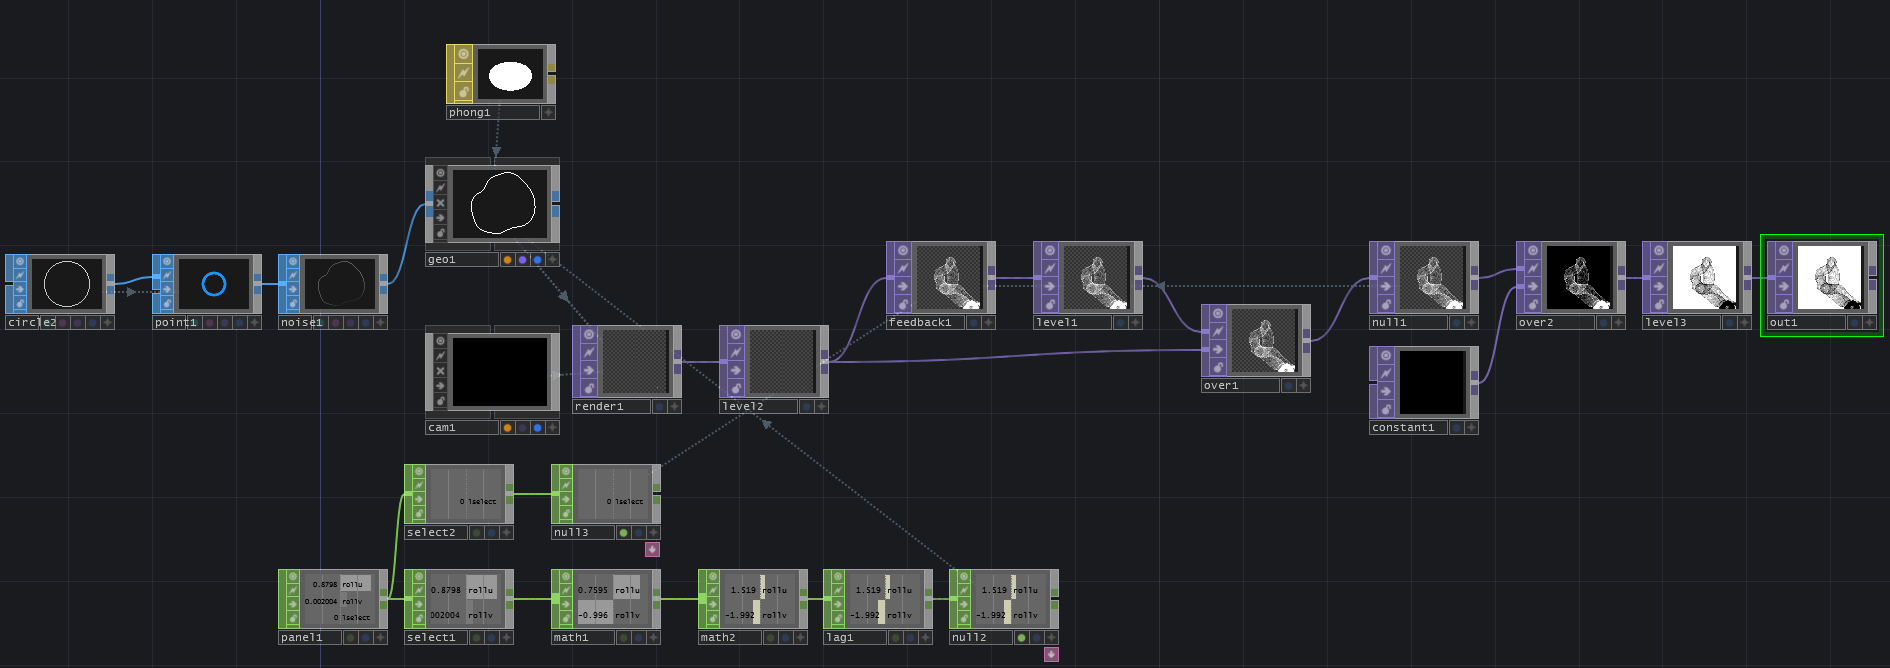
\includegraphics[width=\textwidth]{img/ggForms02.PNG}
  \caption[shortCaption]
  {CAPTION MISSING}
  \label{fig:label}
\end{figure}

\begin{figure}[H]
  \centering
  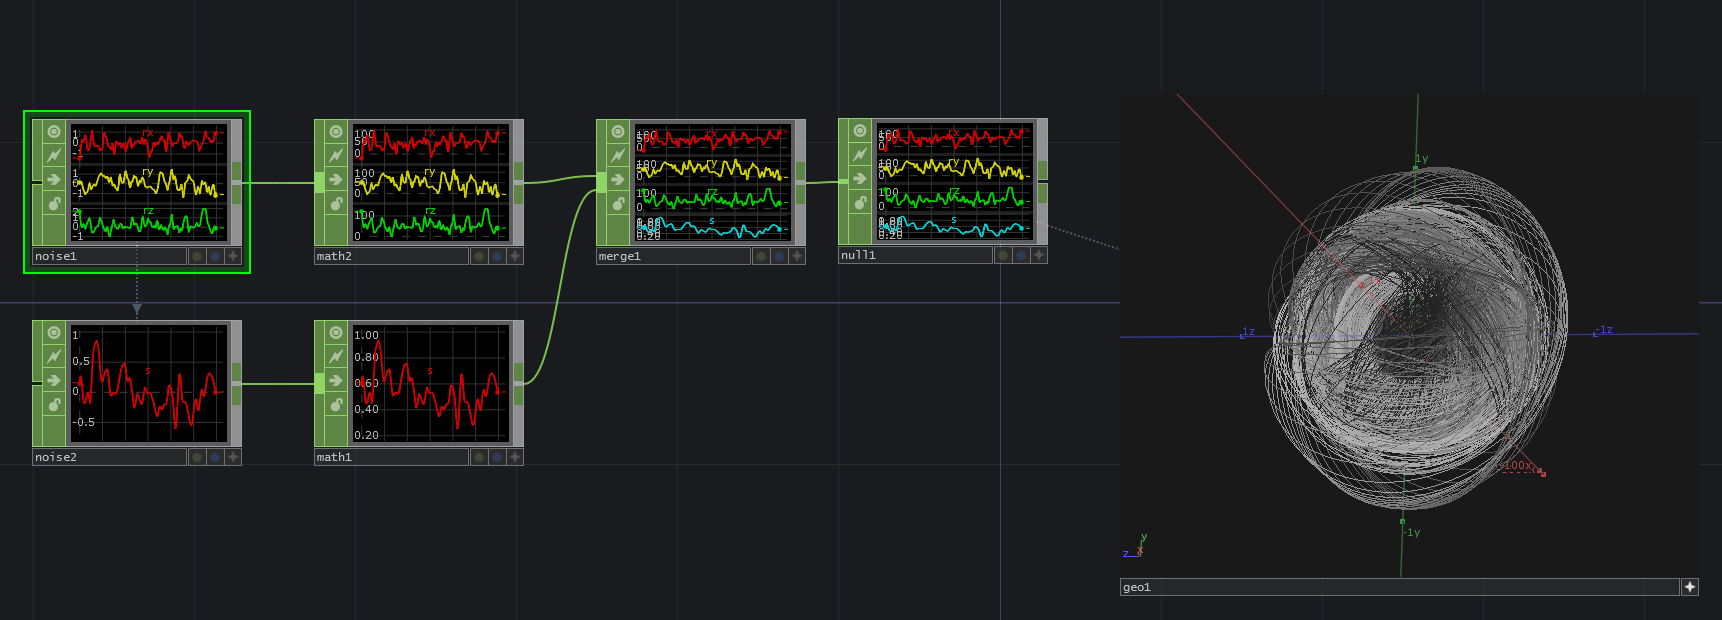
\includegraphics[width=\textwidth]{img/instancing1.PNG}
  \caption[shortCaption]
  {CAPTION MISSING}
  \label{fig:label}
\end{figure}

\begin{figure}[H]
  \centering
  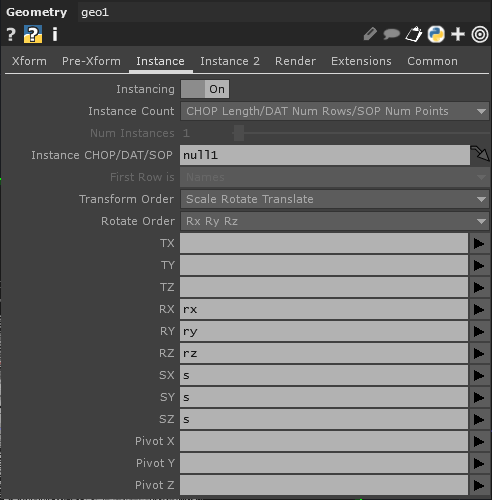
\includegraphics[width=8cm]{img/instancing2.PNG}
  \caption[shortCaption]
  {CAPTION MISSING}
  \label{fig:label}
\end{figure}

\begin{figure}[H]
  \centering
  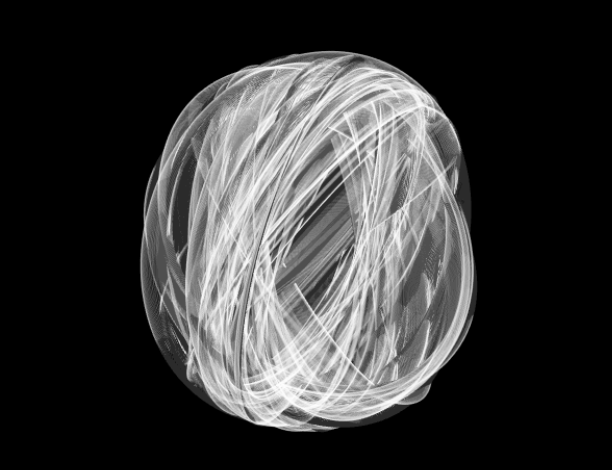
\includegraphics[width=10cm]{img/rings7200.PNG}
  \caption[shortCaption]
  {7200 circles in movement plus some material tweaking}
  \label{fig:label}
\end{figure}

\begin{figure}[H]
  \centering
  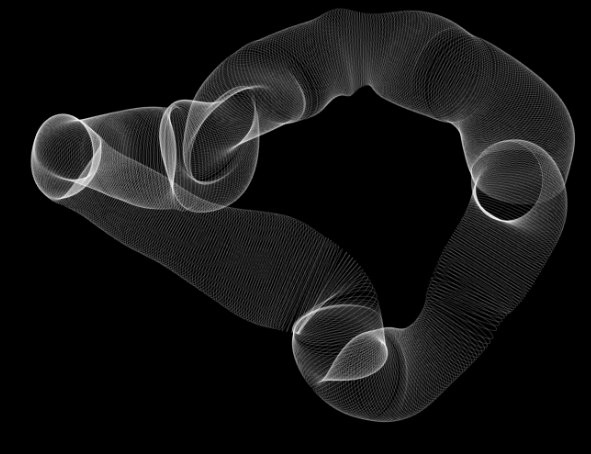
\includegraphics[width=\textwidth]{img/ggForms3d.PNG}
  \caption[shortCaption]
  {Three dimensional version of the generative design noise circle example}
  \label{fig:label}
\end{figure}



\begin{figure}[H]
	\centering
	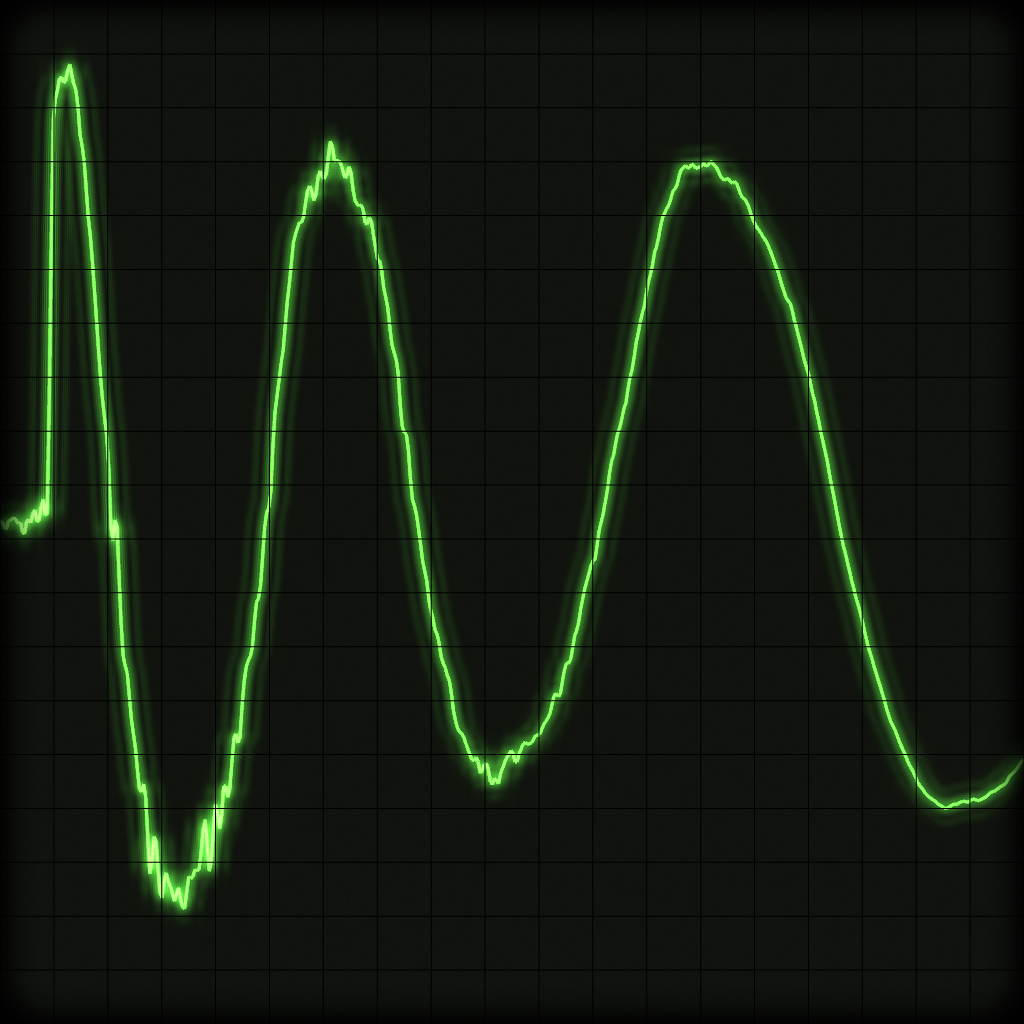
\includegraphics[width=10cm]{img/oscilloscope.png}
	\caption[shortCaption]
	{CAPTION MISSING}
	\label{fig:label}
\end{figure}


\begin{figure}[H]
  \centering
  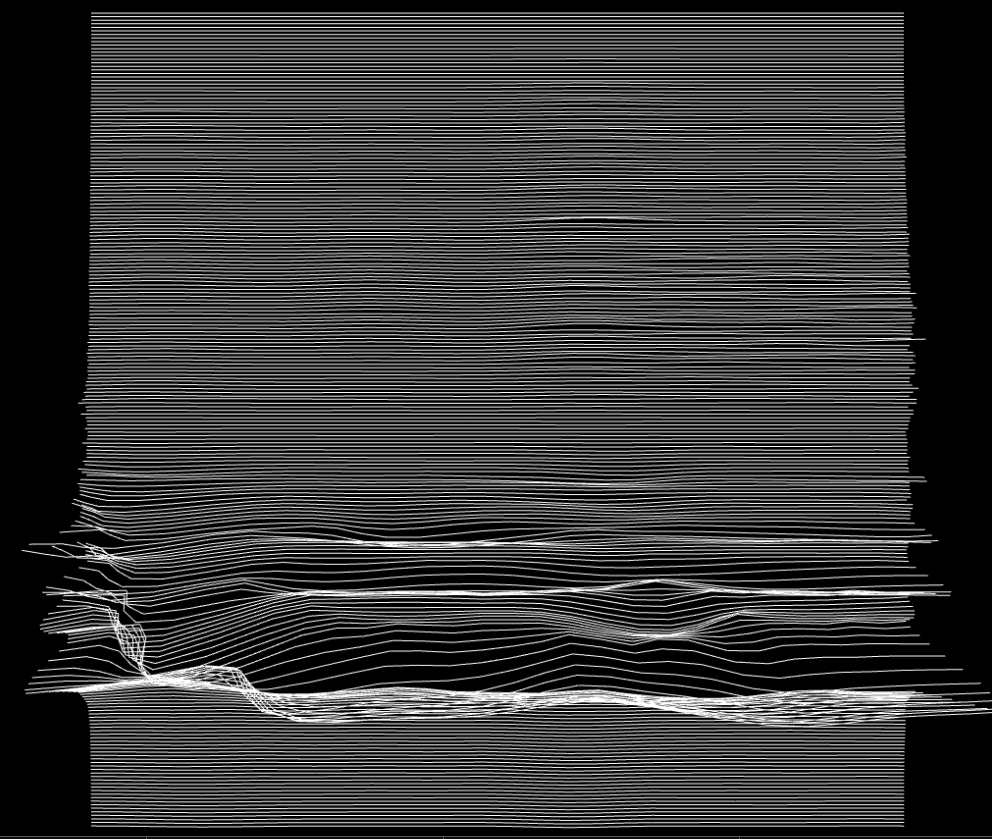
\includegraphics[width=\textwidth]{img/waterfall.PNG}
  \caption[shortCaption]
  {Waterfall plot of an audio spectrum}
  \label{fig:label}
\end{figure}


\begin{figure}[H]
	\centering
	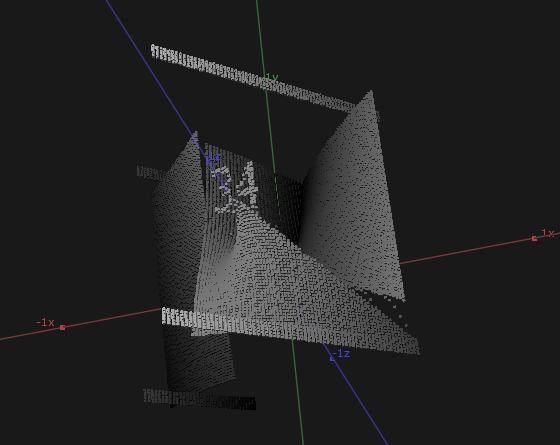
\includegraphics[width=\textwidth]{img/convert2Dto3D.PNG}
	\caption[shortCaption]
	{CAPTION MISSING}
	\label{fig:label}
\end{figure}



\begin{figure}[H]
	\centering
	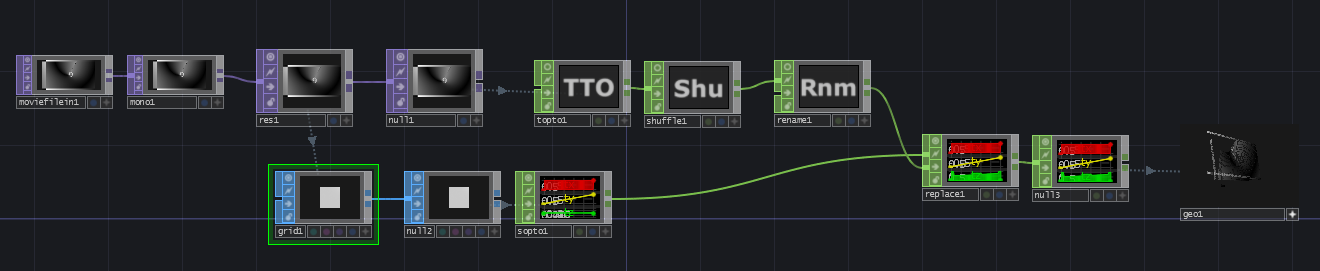
\includegraphics[width=\textwidth]{img/convert2Dto3D2.PNG}
	\caption[shortCaption]
	{CAPTION MISSING}
	\label{fig:label}
\end{figure}



\begin{figure}[H]
	\centering
	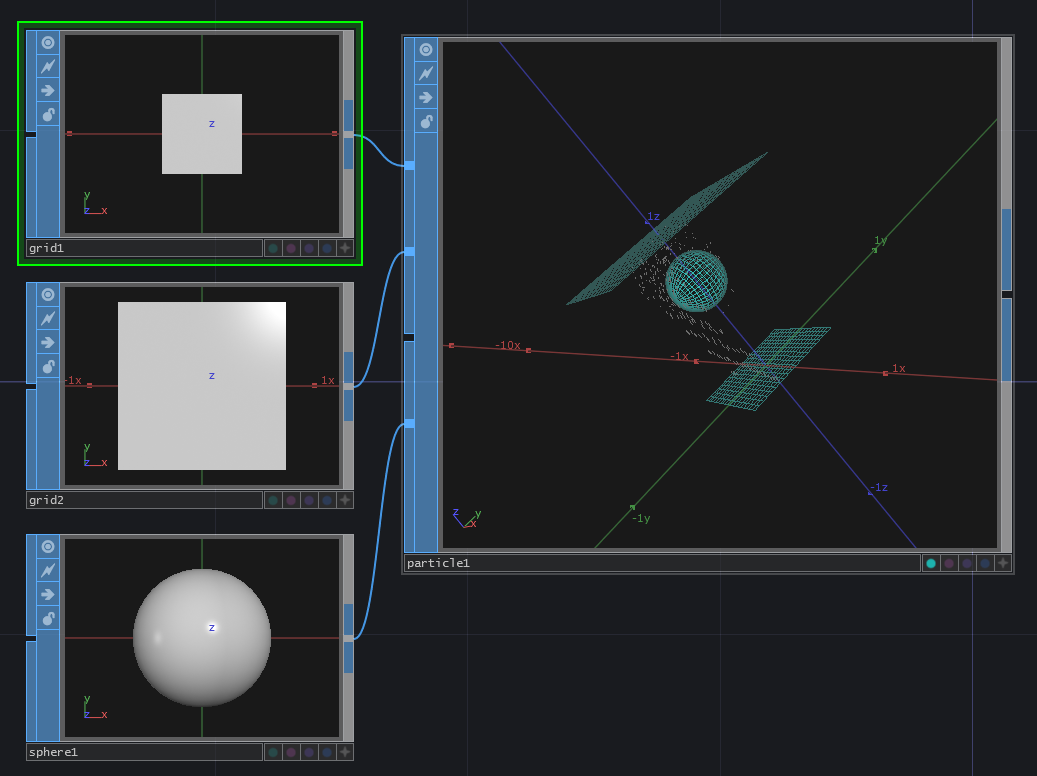
\includegraphics[width=\textwidth]{img/particles1.PNG}
	\caption[shortCaption]
	{CAPTION MISSING}
	\label{fig:label}
\end{figure}



\begin{figure}[H]
  \centering
  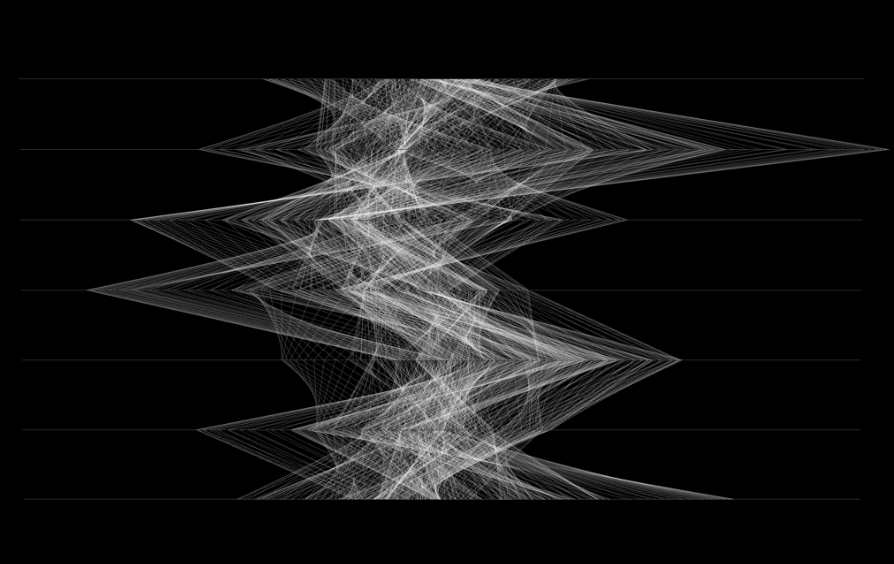
\includegraphics[width=\textwidth]{img/hyperDim.PNG}
  \caption[shortCaption]
  {'parallel Coordinates', a technique for hyperdimensional data visualization}
  \label{fig:label}
\end{figure}


